\includepdf[pages=-]{"Tareas/Hoja 1/Hoja 1"}

\begin{enumerate}[label=\color{red}\textbf{\arabic*)}, leftmargin=*]
	\item \lb{Los siguientes datos corresponden al nivel de glucosa en sangre de diez niños: \[ \begin{array}{|c|c|c|c|c|c|c|c|c|c|}
			\hline
			56 & 62 & 63 & 65 & 65 & 65 & 65 & 68 & 70 & 72\\ \hline
		\end{array} \]}
	\begin{enumerate}[label=\color{red}\alph*)]
		\item \db{Calcula la media, la mediana y la moda. ¿Son parecidas? ¿Por qué?}
		
		$\overline{x},Me,Mo?$
		\[ \begin{array}{|c|c|c|c|c|c|c|}
			\hline
			x_i & f_i & F_i & x_if_i & x_i^2f_i & x_i^3f_i & x_i^4f_i \\ \hline
			56 & 1 & 1 & 56 & 3136 & 175616 & 9834496 \\
			62 & 1 & 2 & 62 & 3844 & 238328 & 14776336 \\
			63 & 1 & 3 & 63 & 3969 & 250047 & 15752961 \\
			65 & 4 & 7 & 260 & 16900 & 1098500 & 71402500 \\
			68 & 1 & 8 & 6 & 4624 & 314432 & 21381376 \\
			70 & 1 & 9 & 70 & 4900 & 343000 & 24010000 \\
			72 & 1 & 10 & 72 & 5184 & 373248 & 26873856 \\ \hline
			& 10 &  & 654 & 42557 & 2793171 & 184031525\\ \hline
		\end{array} \]$\overline{x}=\dfrac{1}{n}\sum x_if_i=\dfrac{651}{10}=\bboxed{65.1}$
		
		Mediana: $\dfrac{n}{2}=\dfrac{10}{2}=5\longrightarrow$ Miramos el volumen de frecuencias acumuladas $(F_i)$, la más próxima por exceso $\longrightarrow\bboxed{Me=65}$
		
		Moda: Moda es el valor con mayor frecuencia acumulada $\longrightarrow\bboxed{\mathrm{Moda}=65}$
		\item \db{Dibuja el diagrama de barras y el gráfico acumulativo de frecuencias.}
		
		
			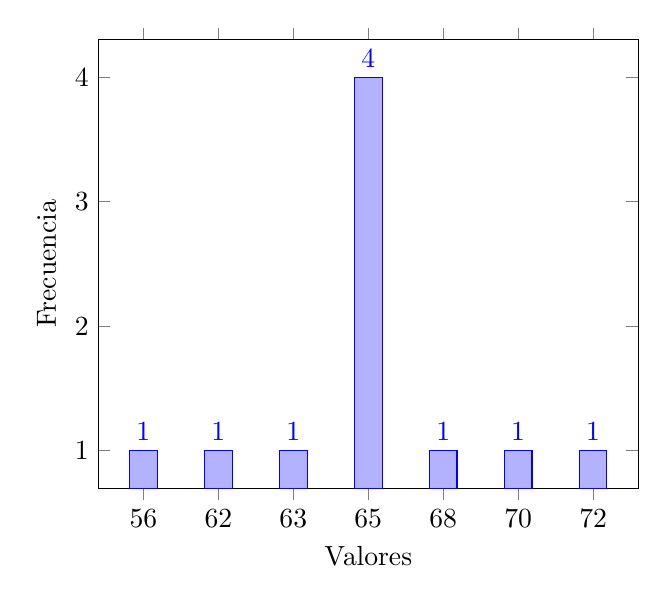
\begin{tikzpicture}
			\begin{axis}[
				ybar,
				xlabel={Valores},
				ylabel={Frecuencia},
				symbolic x coords={56, 62, 63, 65, 68, 70, 72},
				xtick=data,
				nodes near coords,
				nodes near coords align={vertical},
				]
				\addplot coordinates {(56,1) (62,1) (63,1) (65,4) (68,1) (70,1) (72,1)};
			\end{axis}
		\end{tikzpicture}\qquad
		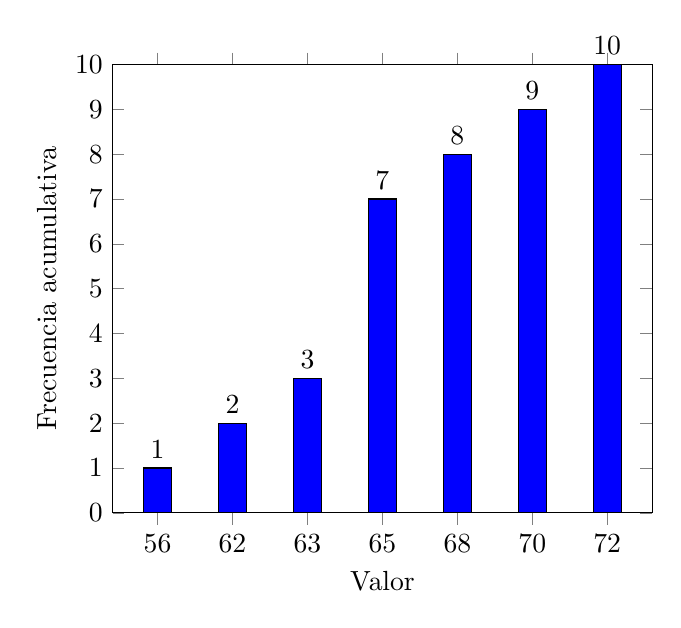
\begin{tikzpicture}
			\begin{axis}[
				ybar,
				ylabel={Frecuencia acumulativa},
				xlabel={Valor},
				ymin=0,
				ymax=10,
				ytick={0,1,2,3,4,5,6,7,8,9,10},
				xtick=data,
				symbolic x coords={56,62,63,65,68,70,72},
				bar width=10pt,
				nodes near coords,
				nodes near coords align={vertical},
				]
				
				\addplot[draw=black,fill=blue] coordinates {
					(56,1)
					(62,2)
					(63,3)
					(65,7)
					(68,8)
					(70,9)
					(72,10)
				};
				
			\end{axis}
		\end{tikzpicture}

		\item \db{Calcula el rango, la varianza y la desviación típica.}
		
		Rango $=x_{\max}-x_{\min}=72-56=\bboxed{16}$\\
		Varianza: \[ s^2=a_2-\overline{x}^2=\dfrac{1}{n}\sum x_i^2f_i-\overline{x}^2=\dfrac{42557}{10}-(65.1)^2=42557-4238.01=\bboxed{17.69} \]
		Desviación típica: \[ s)+\sqrt{s^2}=+\sqrt{17.69}=\bboxed{4.2059} \]
		\item \db{Calcula el coeficiente de variación, el cociente de asimetría y el cociente de apuntamiento. Interpreta sus resultados.}
		
		$\begin{array}{l}
			CV=\dfrac{s}{\overline{x}}=\dfrac{4.2059}{65.1}=0.0646\longrightarrow\bboxed{CV=6.46\%}\\
			CA=\dfrac{m_3}{s^3}\\
			m_3=a_3-3a_2\overline{x}+2\overline{x}^3\\
			a_3=\dfrac{1}{n}\sum x_i^3f_i=\dfrac{2793171}{10}=279317.1\\
			a_2=\dfrac{1}{n}\sum x_i^2f_i=4255.7\\
			m_3=279317.1-3\cdot4255.7\cdot65.1-2\cdot(65.1)^3=-1.103\\
			CA=\dfrac{m_3}{s^3}=\dfrac{-1.103}{(4.2059)^3}=\bboxed{-0.014}<0\longrightarrow\text{Asimetría cola izquierda}\\
			CAp=\dfrac{m_4}{s^4}=\dfrac{988.3217}{312.9361}=\bboxed{3.1583>3}\longrightarrow\text{Leptovértice}\\
			m_4=a_4-4a_3\overline{x}+6a_2\overline{x}^2-3\overline{x}^4=\dfrac{1}{n}\sum(x_i-\overline{x})^4f_i=988.3217\\
		\end{array}$
	\end{enumerate}
	\item \lb{Con el fin de analizar los sueldos de los habitantes de una comarca, se entrevistó a 20 trabajadores en activo que proporcionaron los siguientes valores de sus sueldos brutos anuales (en miles de euros):\[ \begin{array}{|c|c|c|c|c|c|c|c|c|c|}
			\hline
			7 & 9 & 7 & 158 & 11 & 37 & 37 & 31 & 89 & 60 \\ \hline
			98 & 26 & 69 & 41 & 16 & 22 & 1 & 7 & 29 & 125\\ \hline
		\end{array} \]}
	\begin{enumerate}[label=\color{red}\alph*), leftmargin=*]
		\item \db{Para los datos \textbf{sin} agrupar calcula la media aritmética, la mediana, los cuartiles, la desviación típica, la varianza, el coeficiente de variación y el rango intercuartílico. Compara los valores de la media y la mediana, ¿son parecido o distintos?, ¿a qué se debe?}
		
		$\overline{x}=\dfrac{\sum x_i}{n}=\dfrac{7+9+\cdots+125}{20}=44$
		
		$Me=\dfrac{\chi_{10}+\chi_{11}}{2}$ porque $n=20$ (par)
		
		Ordeno datos de menor a mayor: \[ 1~~7~~7~~7\underset{\color{lightblue}\begin{subarray}{c}
				\downarrow\\
				Q_1=\frac{9+11}{2}=10
		\end{subarray}}{\bboxed{9~~11}}16~~22~~26\underset{\color{lightblue}\begin{subarray}{c}
		\downarrow\\
		Me=\frac{29+31}{2}=30
	\end{subarray}}{\bboxed{29~~31}}373~~37~~41\underset{\color{lightblue}\begin{subarray}{c}
	\downarrow\\
	Q_3=\frac{60+69}{2}=64.5
\end{subarray}}{\bboxed{60~~69}}89~~98~~125~~158 \]

\begin{wrapfigure}{r}{0.5\textwidth}
	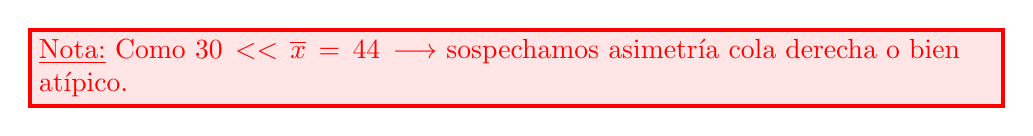
\begin{tikzpicture}
		\node[red, draw=red, fill=red!10, line width=1.5, text width=\textwidth] {\underline{Nota:} Como $30<<\overline{x}=44\longrightarrow$ sospechamos asimetría cola derecha o bien atípico.};
	\end{tikzpicture}
\end{wrapfigure}

$Q_1=1^\circ$ Cuartil$\longrightarrow$ Lo que obtenemos como la mediana de los datos por debajo de la mediana (excluida esta).
\begin{itemize}[label=\color{red}\textbullet, leftmargin=*]
	\item \color{lightblue}Histograma
\end{itemize}
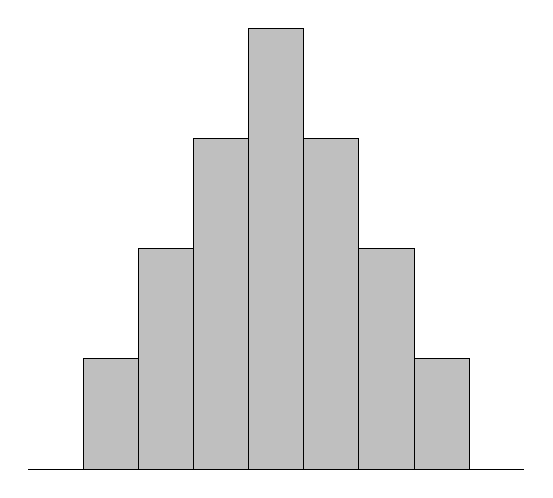
\begin{tikzpicture}[scale=0.7]
	\draw (0,0) -- (9,0);
	\draw[draw=black, fill=lightgray] (1,0) rectangle (2,2);
	\draw[draw=black, fill=lightgray] (2,0) rectangle (3,4);
	\draw[draw=black, fill=lightgray] (3,0) rectangle (4,6);
	\draw[draw=black, fill=lightgray] (4,0) rectangle (5,8);
	\draw[draw=black, fill=lightgray] (5,0) rectangle (6,6);
	\draw[draw=black, fill=lightgray] (6,0) rectangle (7,4);
	\draw[draw=black, fill=lightgray] (7,0) rectangle (8,2);
\end{tikzpicture}\qquad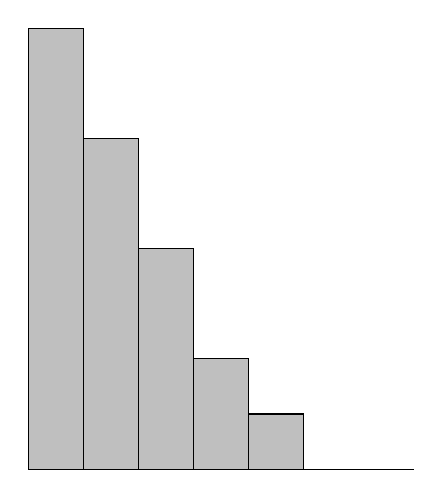
\begin{tikzpicture}[scale=0.7]
\draw (0,0) -- (7,0);
\draw[draw=black, fill=lightgray] (0,0) rectangle (1,8);
\draw[draw=black, fill=lightgray] (1,0) rectangle (2,6);
\draw[draw=black, fill=lightgray] (2,0) rectangle (3,4);
\draw[draw=black, fill=lightgray] (3,0) rectangle (4,2);
\draw[draw=black, fill=lightgray] (4,0) rectangle (5,1);
\end{tikzpicture}

Si la distribución es simétrica ¿$\overline{x}, Me$, Moda?

$\begin{array}{l}
	s_x^2=\dfrac{\displaystyle\sum_{i=1}^{n}(x_i-\overline{x}^2)}{n}=\overline{x^2}-(\overline{x})^2\\
	\overline{x^2}=\dfrac{\sum x_i^2}{n}=\dfrac{7^2+9^2+\cdots+125^2}{20}=\dfrac{77491}{20}\\
	s_x^2=\dfrac{77491}{20}-(44)^2=1938.55\longrightarrow s_x=\sqrt{s_x^2}=44.03
\end{array}$
\item \db{Dibuja de forma detallada el diagrama de caja y bigotes del conjunto de datos. Comentar las características más relevantes: ¿los datos se distribuyen de forma simétrica o asimétrica?, ¿cuál es el intervalo de valores admisibles, es decir, dónde se encuentran los no atípicos?, ¿existen valores atípicos?}
\begin{itemize}
	\item $LSA=Q_3+1.5\cdot RIC=64.5+1.5\cdot54.5=145.25$
	\item $LIA=Q_1+1.5\cdot RIC=10-1.5\cdot 54.5=-71.75$
\end{itemize}

\begin{center}
	\begin{tikzpicture}
		\draw (3,{1/20}) -- (3,{125/20});
		\draw (0,0) -- (0,8);
		\draw (0,0) -- (8,0);
		\foreach \x in {0,20,40,...,160}{
		\node[left] at (0,{\x/20}) {\x};
		}
		\draw[fill=lightgray] (1,0.5) rectangle (5, {64.5/20});
		\draw[-latex] (1,1.5) -- (5.5,1.5) node[right] {Me};
		\draw[-latex] (5,0.5) -- (5.5,0.5) node[right] {$Q_1$};
		\draw[-latex] (5,{64.5/20}) -- (5.5,{64.5/20}) node[right] {$Q_3$};
		\draw (2.8, {125/20}) -- (3.2,{125/20}) node[lightblue, right] {$\max(x_i)$ en zona admisible $=125$};
		\draw (2.8, {1/20}) -- (3.2,{1/20}) node[lightblue, below right] {$\min(x_i)$ en zona admisible $=1$};
		\draw[dashed] (0,7.2) -- (8,7.2);
		 \draw[fill=lightgray] (3,{158/20}) circle (0.2cm);
		 \draw[-latex] (3.2, {158/20}) -- (4,{158/20}) node[lightblue, right] {Outlier $=158$};
	\end{tikzpicture}
\end{center}
\item \db{Si queremos agrupar los datos en clases, ¿cuántas clase deberíamos realizar?, ¿de qué amplitud?}

$d=\dfrac{\max(x_i)-\min(x_i)}{k}=\dfrac{158-1}{5}=31.4$
\item \db{Realizar la agrupación de los datos en 5 clases y determinar la tabla de frecuencias absolutas, relativas y sus acumuladas. ¿Qué porcentaje de individuos de la muestra cobran un salario menor o igal a 96000 euros brutos anuales?, ¿y entre 64000 y 128000?}

\begin{tabular}{|c|c|c|c|c|}
	\hline
	Clases & $f_i$ & $F_i$ & $h_i$ & $H_i$ \\
	\hline
	[0,32]& 11 & 11 & $\dfrac{11}{20}$  & $\dfrac{11}{20}$ \\
	\hline
	(32,64]& 4 & 15 & $\dfrac{4}{20}$ & $\dfrac{15}{20}$ \\
	\hline
	(64,96]& 2 & 17 & $\dfrac{2}{20}$ & $\dfrac{17}{20}$ \\
	\hline
	(96,128]& 2 & 19 & $\dfrac{2}{20}$ & $\dfrac{19}{20}$ \\
	\hline
	(128,160]& 1 & 20 & $\dfrac{1}{20}$ & 1 \\
	\hline
	& 20 &  &  &  \\
	\hline
\end{tabular}

$\dfrac{17}{20}=0.85\longrightarrow85\%$ cobran $\le96000$€

$100\cdot\left(\dfrac{19}{20}-\dfrac{15}{20}\right)=20\%$ cobran entre 64000 y 128000
\item \db{Calcular la media aritmética y la varianza para los datos agrupados en el apartado anterior. Determinar la clase que contiene a la mediana, la clase modal y proporciona sus marcas de clase. Compara la magnitud de las tres medidas de centralización (media, mediana y moda)}

$\begin{array}{l}
	\overline{x}=\dfrac{16\cdot11+48\cdot4+80\cdot2+112\cdot2+144\cdot1}{20}=44.8\\
	Me=\dfrac{\chi_{10}+\chi_{11}}{2}\in[0,32]
\end{array}$
	\end{enumerate}
	\item \begin{enumerate}[label=\color{red}\alph*)]
		\item \lb{Sea $\{x_1,x_2,\dots,x_{100}\}$ una muestra de media aritmética 21.5 y sean $x_{101}=22,x_{102}=19,x_{103}=20.5$ tres observaciones más. Calcular la media aritmética de la nueva muestra $\{x_1,x_2,\dots,x_{100},x_{101},x_{102},x_{103}\}$}
		
		$\{x_1,x_2,\dots,x_{100}\}$\\
		$\{x_1,x_2,\dots,x_{100},22,19,20.5\}\longrightarrow\overline{x}=$¿?\\
		$\overline{x}=\dfrac{1}{n}\sum_{i=1}^{103}x_if_i=\dfrac{1}{103}\left(\sum_{i=1}^{100}x_if_i+\sum_{i=1}^{103}x_if_i\right)=\dfrac{1}{103}\left(100\cdot21.5+22+19+20.5\right)=21.4709$
		\item \lb{Sea $\overline{x}$ la media aritmética de la muestra $\{x_1,x_2,\dots,x_n\}$ y sea $\overline{y}$ la media aritmética de la muestra $\{y_1,y_2,\dots,y_m\}$. ¿Cuál será la media aritmética de la unión de ambas muestras?}
		
		$\begin{rcases}
			\{x_1,x_2,\dots,x_n\}\longrightarrow\overline{x}\\
			\{y_1,y_2,\dots,y_m\}\longrightarrow\overline{y}
		\end{rcases}\{x_1,x_2,\dots,x_n,y_1,y_2,\dots,y_m\}\longrightarrow$¿$\overline{z}$?
		
		$z=\dfrac{1}{n+m}\sum_{i=1}^{n+m}z_if_i=\dfrac{1}{n+m}\left[\sum_{i=1}^{n}x_if_i+\sum_{i=1}^{m}y_if_i\right]=\dfrac{1}{n+m}\left[n\cdot\overline{x}+m\cdot\overline{y}\right]$
		
		$\bboxed{z=\dfrac{m\cdot\overline{x}+m\cdot\overline{y}}{n+m}}$
	\end{enumerate}
	\item \lb{Probar que la media aritmética y la mediana son operadores lineales, es decir, si tenemos una muestra $\{x_1,x_2,\dots,x_n\}$ con media $\overline{x}$ y cada una de las observaciones $x_i$ la multiplicamos por una constante $"a"$ y le sumamos otra constante $"b"$, es decir, obtenemos una nueva muestra $ \{y_1,y_2,\dots,y_n\}$ donde $y_I=ax_i+b\;\forall i=1,\dots,n$, entonces la media de la nueva muestra $\overline{y}$, verifica $\overline{y}=a\overline{x}+b$ (igual con la mediana).}
	
	$\underset{\begin{subarray}{c}
			\downarrow\\
			\text{media $=\overline{x}$}
	\end{subarray}}{\{x_1,x_2,\dots,x_n\}}\longrightarrow\underbrace{\{\underbrace{ax_1+b}_{y_1},\underbrace{ax_2+b}_{y_2},\dots,\underbrace{ax_n+b}_{y_n}\}}_{\text{¿media $(y)=\overline{y}=a\overline{x}+b$?}}$

$\overline{y}=\dfrac{\sum_{i=1}^{n}y_i}{n}=\dfrac{\sum_{i=1}^{n}(ax_i+b)}{n}=\dfrac{\sum_{i=1}^{n}ax_i+\sum_{i=1}^{n}b}{n}=\dfrac{a\sum x_i+b_n}{n}=a\cdot\lbb{\dfrac{\sum x_i}{n}}{\overline{x}}+b=a\overline{x}+b$

¿Qué pasa con las medianas?

Ordenamos datos de $\{x_1,\dots,x_n\}$ de menor a mayor.\\
$x_{(1)}\le x_{(2)}\le\dots\le x_{(n)}\longrightarrow Me_{(x)}=x_{\left(\frac{n+1}{2}\right)}$ (supongo $n$ impar)\\
\begin{itemize}
	\item Si $a>0\longrightarrow y_{(1)}\le y_{(2)}\le \dots\le y_{(n)}\longrightarrow Me_{(y)}=y_{\left(\frac{n+1}{2}\right)}=\bboxed{ax_{\left(\frac{n+1}{2}\right)}+b}$
	\item Si $a<0\longrightarrow$ Se invierte el orden pero la posición central la ocupa el mismo dato.
\end{itemize}
\item \lb{Sea $\{x_1,x_2,\dots,x_n\}$ una muestra con media $\overline{x}$ y varianza $s_X^2$. Si cada una de las observaciones $x_i$ la multiplicamos por una constante $"a"$ (con $a\neq0$) y le sumamos otra constante $"b"$, es decir, obtenemos una nueva muestra $\{y_1,y_2,\dots,y_n\}$ donde $y_i=ax_i+b\;\forall i=,\dots,n$}

$\{x_1,\dots,x_n\}$ aumenta con moda $\overline{x}$ y varianza $s_X^2$. Sea $\{y_1=ax_1+b,y_2=ax_2+b,\dots,y_n=ax_n+b\}$

\begin{enumerate}[label=\color{red}\alph*)]
	\item \db{¿Qué relación existe entre la varianza de la $Y(S_Y^2)$ y la varianza de la $X(S_X^2)$?}
	
	$S_X^2=\dfrac{\sum_{i=1}^{n}(x_i-\overline{x})^2}{n}$\\
	$S_Y^2=\dfrac{\sum_{i=1}^{n}(y_i-\overline{y})^2}{n}=\dfrac{\sum_{i=1}^{n}\left((ax_i+b)-(a\overline{x}+b)\right)^2}{n}=\dfrac{\sum_{i=1}^{n}\left(a^2(x_i-\overline{x})\right)^2}{n}=a^2\cdot\dfrac{\sum_{i=1}^{n}(x-i-\overline{x})^2}{n}=a^2\cdot S_X^2$
	\item \db{¿Qué relación existe entre la desviación típica de la $Y(S_Y)$ y la desviación típica de la $X(S_X)$?}
	
	$S_Y=\sqrt{a^2\cdot S_X^2}=\bboxed{|a|\cdot S_X}$
\end{enumerate}
\end{enumerate}
